\section{Volumetric displays}

Volumetric displays \cite{1492264} are a promising technology that offers a captivating three-dimensional viewing experience. By emitting light for each voxel, or volume element, in a 3D space, these displays transcend the limitations of traditional 2D planes, providing a truly immersive 3D effect. This innovative approach enables the accurate representation of virtual 3D objects, including focal depth, motion parallax, and vergence, which refers to the rotation of a viewer's eye to fixate on the same point they are focusing on. Moreover, volumetric displays allow multiple users to view the same display from different angles, providing unique perspectives of the same object.

\subsection{Swept Volume Displays}
Swept volume displays represent one category of volumetric displays. They employ a moving 2D display to create a 3D image. This is achieved by moving the 2D display through a 3D space and emitting light from the display at each point. Common techniques for achieving this include using a rotating mirror \cite{10.1117/12.480930}, emitting screen typically an LED \cite{Gately:11}, or transparent projector screen \cite{keane_volumetric_2016}. There currently exist commercial products that implement this as can be seen in Fig~\ref{fig:voxon} and Fig~\ref{fig:brightbox}.

\begin{invisBox}
  
  \pictureBox[label={fig:voxon}]{The VXR4612 3D Volumetric Display, a projector-based persistence of vision display produced by Voxon Photonics. \cite{voxon2}}{
    \adjustbox{height=4cm, keepaspectratio}{
      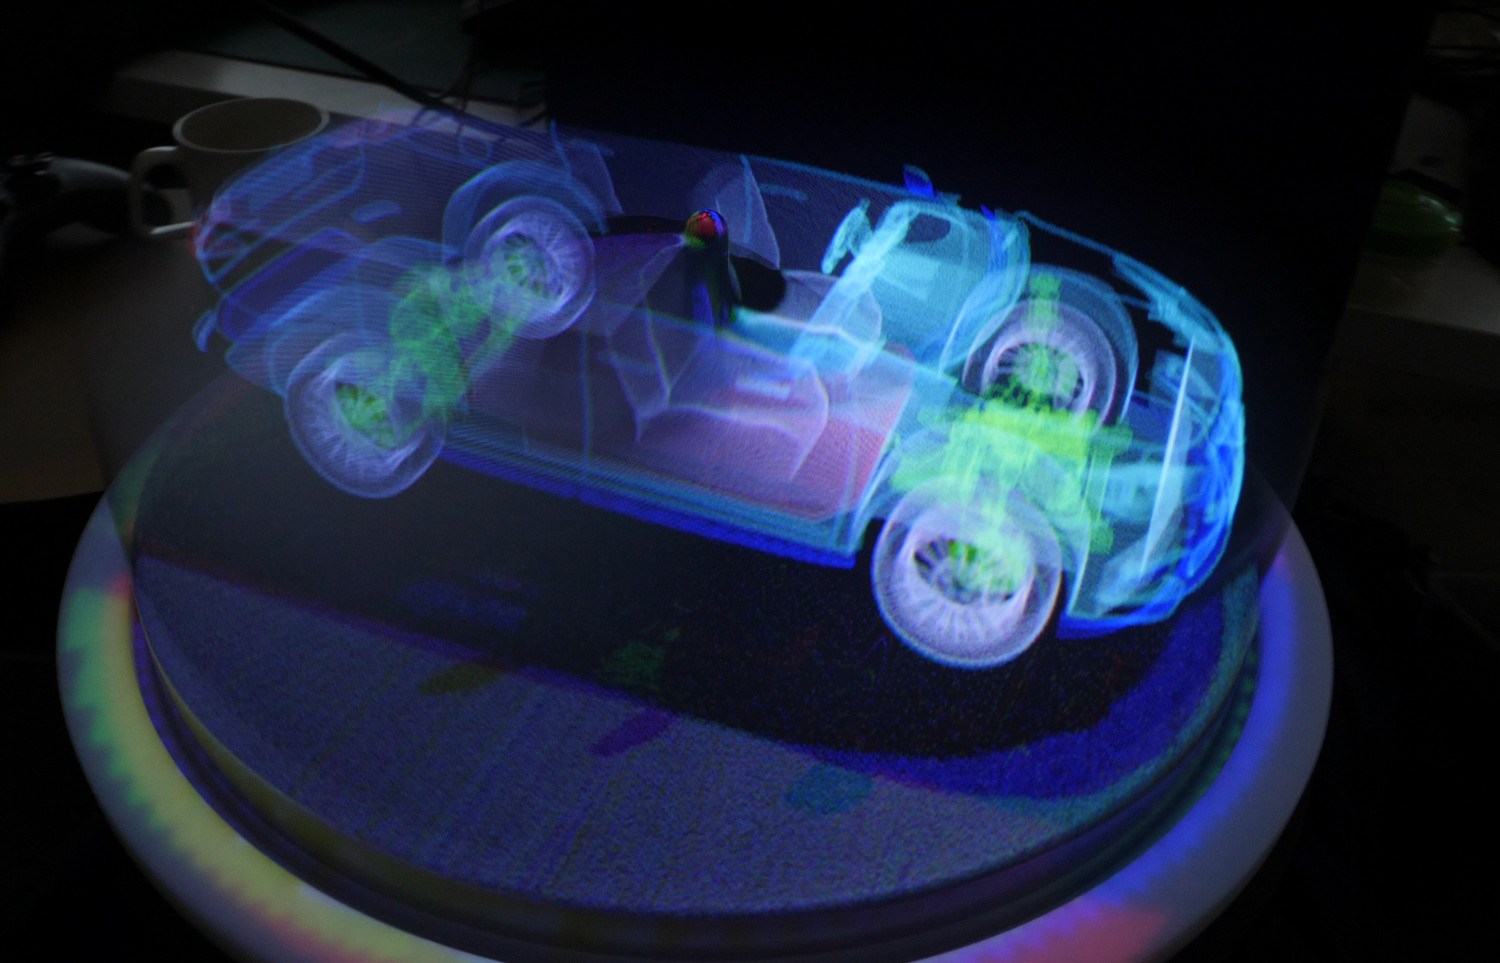
\includegraphics{./background/figures/3d/voxon.jpg}
    }
  }
  \hfill
  \pictureBox[label={fig:brightbox}]{A Volumetric Display / Holographic Signage, an LED-based persistence of vision display produced by Brightvox Inc. \cite{brightvox_2023}}{
  \adjustbox{height=4.5cm, keepaspectratio}{
    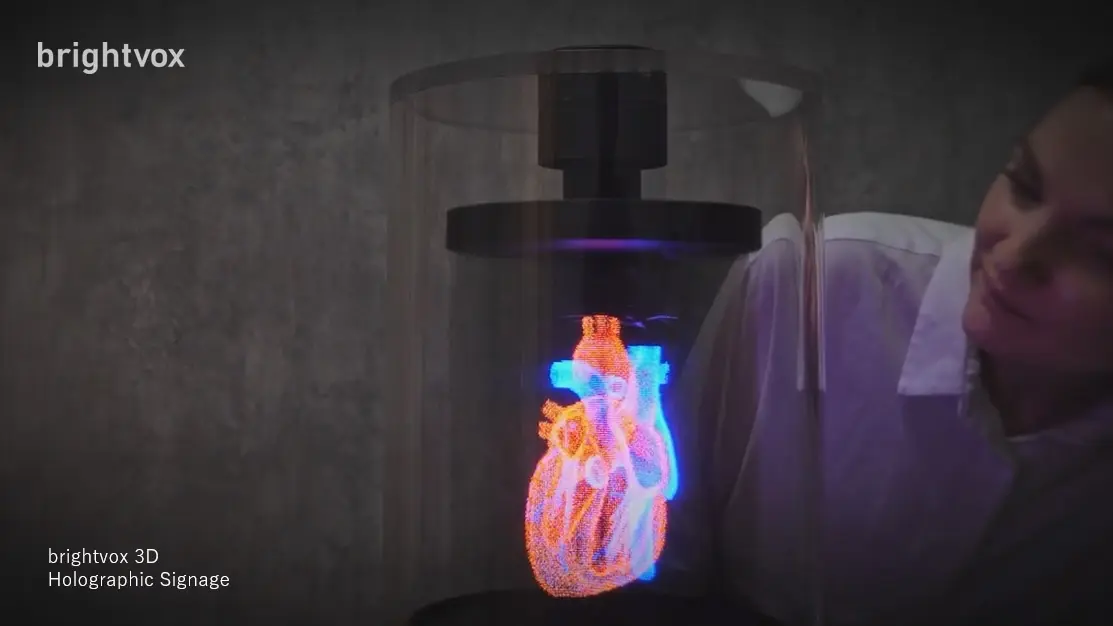
\includegraphics{./background/figures/3d/brightvox.png}
    }
  }
\end{invisBox}

\subsection{Static Volume Displays}
Static volume displays are another category of volumetric displays. They employ a static 3D display to create a 3D image. This is achieved by emitting light from the display at each point in a 3D space. Techniques for achieving this range from using a 3D array of LEDs \cite{10.1145/2341931.2341937}, lasers and phosphorus gas \cite{https://doi.org/10.1002/anie.202003160}, or a transparent laser-induced damaged medium that can be projected into \cite{10.1145/1179849.1179982}. There has been research into photon-activated dye \cite{Patel2017} and even quantum dot-based displays \cite{Hirayama2015}.

\subsection{Trapped Particle Displays}
Acoustic Trapping Displays displays are a relatively new category of volumetric displays. They employ a 3D array of particles that are suspended in air using acoustic levitation. \cite{10.1063/1.5113467} \cite{Hirayama2019} This is achieved by using an array of ultrasonic transducers to create a standing wave that can trap particles in the nodes of the wave. By moving the nodes of the wave through a 3D space and illuminating the particles with light, a 3D image can be created. This technique is still in its infancy and can struggle to provide a convincing persistence of vision effect. Another direction some researchers have taken is to use a photophoretic trap to trap particles in air \cite{Smalley2018}.

\subsection{Issues}

Volumetric displays often require custom/cutting-edge hardware (e.g. extremely high refresh rate projectors,  transparent micro LEDs) which makes them expensive, difficult to manufacture and not widely available. For example, the Voxon VX1, one of the few if only commercially available volumetric displays costs, \$11,700 USD \cite{noauthor_products_nodate} per unit. \\

Volumetric displays are also held back by their inherent high bandwidth requirements: To render objects in real-time at equivalent resolutions to current 2D displays while taking a raw voxel stream (as opposed to calculating voxels on hardware from primitive shapes) has an extremely high bandwidth requirement. If we want to render at \texttt{60fps} on a $4096 \times 2160 \times 1080$ voxel display with \texttt{24 bit} color, it would require a bandwidth of $1.37 \times 10^3$ bits per second/13.7 terabits per second which is orders of magnitude higher than what a normal display requires. To achieve that currently would require about 170 state-of-the-art Ultra High Bit Rate (UHBR) (80 gigabit) DisplayPort cables simultaneously. It was predicted in 2021 \cite{LAM2021050011} that due to these limitations and based on the historic trends of bandwidth in commercially available displays, volumetric displays will only become commercially feasible in 2060 at the earliest. There are ways to reduce this bandwidth requirement through compression and other techniques \cite{4487481} but this still provides a major issue. \\

\subsection{Volumetric Screen Simulations}
Because of these issues, there has been some research into simulating volumetric displays. One commonly used method is by using so-called fish tank virtual reality (FTVR) display \cite{10.1145/169059.169066} which has been commonly used to simulate volumetric displays, \cite{10.1145/3281505.3281540}, \cite{Zabarauskas2012}. A FTVR comprises a singular or set of 2D displays that are positioned in front of a user. The viewer's eyes are tracked in 3D space the image on the displays is adjusted accordingly so that there appears to be a 3D image in front of them. This is a relatively cheap and easy way to simulate a volumetric display, but it has some major drawbacks. The user is limited to a single focal depth and the user is limited to a single vergence (This can be fixed by wearing glasses to filter different images to each eye providing a stereo view \cite{5701756}). This system is also limited to just a single user at a time unless image filtering is used. 

Another approach that has been taken has been to take advantage of VR headsets. VR headsets are a relatively cheap and easy way to simulate a volumetric display. They are also able to provide a stereo view and can be used by multiple users at once \cite{10.1145/3290605.3300763}.